\documentclass[tikz]{standalone}
\usetikzlibrary{arrows.meta,positioning}

\begin{document}
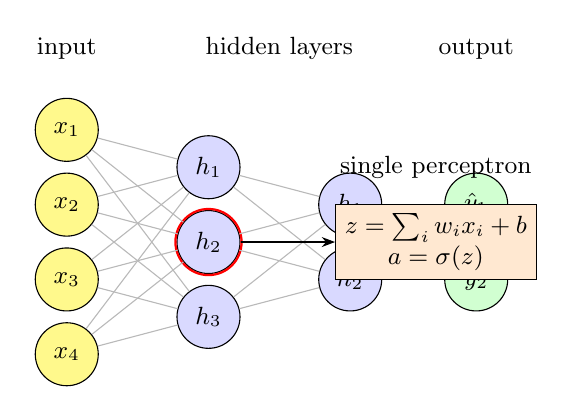
\begin{tikzpicture}[
  >=Stealth,
  neuron/.style={circle,draw,minimum size=8mm,inner sep=0},
  every node/.style={font=\small},
]
  \foreach \ell/\x/\n/\fill in {0/0/4/yellow!45,1/1.8/3/blue!15,2/3.6/2/blue!15,3/5.2/2/green!18} {
    \foreach \i in {1,...,\n} {
      \pgfmathsetmacro{\y}{(\n-1)/2*.95-(\i-1)*.95}
      \node[neuron,fill=\fill] (L\ell-\i) at (\x,\y) {};
    }
  }
  \foreach \l/\n/\sym in {0/4/x,1/3/h,2/2/h}
    \foreach \i in {1,...,\n} \node at (L\l-\i) {$\sym_{\i}$};
  \foreach \i in {1,...,2} \node at (L3-\i) {$\hat y_{\i}$};
  \draw[red,thick] (L1-2) circle (4.2mm);

  \foreach \a/\na/\b/\nb in {0/4/1/3,1/3/2/2,2/2/3/2}
    \foreach \i in {1,...,\na}
      \foreach \j in {1,...,\nb}
        \draw[gray!55] (L\a-\i) -- (L\b-\j);

  \node[above] at (0,2.2) {input};
  \node[above] at (2.7,2.2) {hidden layers};
  \node[above] at (5.2,2.2) {output};
  \node[draw,fill=orange!18,align=center,right=1.2cm of L1-2] (p)
    {$z=\sum_i w_i x_i+b$\\$a=\sigma(z)$};
  \draw[->] (L1-2) -- (p);
  \node[above=2mm of p] {single perceptron};
\end{tikzpicture}
\end{document}
